\documentclass{article}

\usepackage[left=3cm,right=3cm,top=2cm,bottom=2cm]{geometry}
\usepackage{xetexko}
\usepackage{listing}
\usepackage{graphicx}

\begin{document}
    \title{<컴퓨터 프로그래밍 3> 실습보고서 \\ \large [제 01 주] 일차방정식}
    \date{\today}
    \author{201704150 허강준}

    \maketitle

    \newpage

    \tableofcontents

    \newpage

    \section{프로그램 명세}

    \subparagraph{\normalfont본 실습 보고서는 <컴퓨터 프로그래밍 3> 강의의 제 01주차 실습 과제인 일차 방정식 프로그램의 구현과 그 실행 결과의 분석에 대해 다룬다.}

    \subsection{설계}

    \subparagraph{\normalfont이 프로그램은 진입점으로부터 \texttt{App} 이라는 모듈을 호출하며, 이 모듈을 중심으로 \texttt{AppView} 및 \texttt{Calculator}와 같은 모듈과 공통 정의 매크로로 이루어진다. 
    코드 제어는 \texttt{App} 에 정의된 \texttt{App\_Start} 가 가져가며, 모든 사용자 정의 루틴은 이 안에서 실행되도록 한다.}

    \subsection{함수 명세}

    \subparagraph{\normalfont모든 프로시져들은 리턴 형 (\texttt{void})를 생략한다.}

    \paragraph{\large\texttt{int main(void)} \tiny Main.c, Ln 10}

    \subparagraph{\normalfont프로그램의 진입점이다. \texttt{App\_Start}를 호출한다.}

    \paragraph{\large\texttt{int App\_Start(void)} \tiny App.h, Ln 9}

    \subparagraph{\normalfont\texttt{App} 모듈의 진입점이다. 모든 동작은 이 안에서 실행된다.}
    
    \paragraph{\large\texttt{AppView\_out\_msg\_startSolvingLinearEquation(void)} \tiny AppView.h, Ln 7}

    \subparagraph{\normalfont\texttt{<<< 일차방정식 풀이를 시작합니다 >>>} 라는 메세지를 출력한다. \texttt{App} 모듈 시작 시 호출된다.}

    \paragraph{\large\texttt{AppView\_out\_msg\_endSolvingLinearEquation(void)} \tiny AppView.h, Ln 8}

    \subparagraph{\normalfont\texttt{<<< 일차방정식 풀이를 종료합니다 >>>} 라는 메세지를 출력한다. \texttt{App} 모듈 시작 시 호출된다.}

    \paragraph{\large\texttt{AppView\_out\_showLinearEquation(float c0, float c1)} \tiny AppView.h, Ln 9}
    
    \subparagraph{\normalfont 두 개의 \texttt{float} 값을 받아 현재 일차방정식이 어떻게 구성되어있는지 사용자에게 출력한다.}

    \paragraph{\large\texttt{AppView\_out\_showRoot(float root)} \tiny AppView.h, Ln 10}

    \subparagraph{\normalfont 인자로 제공된 \texttt{float} 값을 받아 일차방정식의 해를 출력한다.}

    \paragraph{\large\texttt{AppView\_out\_msg\_error\_firstOrderTermCoefficientIsZero(void)} \tiny AppView.h, Ln 11}

    \subparagraph{\normalfont 1차항의 계수가 0임이 잘못되었음을 알리는 오류메세지를 출력한다.}

    \paragraph{\large\texttt{bool AppView\_in\_getSolvingRequest(void)} \tiny AppView.h, Ln 12}

    \subparagraph{\normalfont 사용자로부터 방정식을 풀 것인지 묻는 메세지를 출력하여 입력을 받는다. \texttt{y} 나 \texttt{Y}를 입력받을 경우 \texttt{true}를, 그 외의 경우 \texttt{false}를 리턴한다.}

    \paragraph{\large\texttt{AppView\_in\_getCoefficient(float* c0, float* c1)} \tiny AppView.h, Ln 13}

    \subparagraph{\normalfont 사용자로부터 계수로 사용할 두개 값을 입력받는다. 이때 저장은 인자로 전달받은 두개의 \texttt{float} 포인터를 통해 저장한다.}

    \paragraph{\large\texttt{float Calculator\_SolveEquation(float c0, float c1)} \tiny Calculator.h, Ln 4}

    \subparagraph{\normalfont 2개의 32비트 부동소숫점 값을 받아 해를 계산한 후 리턴한다.}

    \paragraph{MACRO \large\texttt{F32Abs(f0)} \tiny Macros.h, Ln 6}

    \subparagraph{\normalfont인자로 전달된 32비트 부동소수점 값의 절댓값을 산출한다. IEEE-754에 정의된 단정밀도 부동소숫점의 정의에 따라, MSB의 값을 Bitwise-AND를 통하여 0으로 만든다. 이때 \texttt{f0}와 Bitwise-AND 되는 operand는 \texttt{0x7fffffff}이다.}

    \paragraph{MACRO \large\texttt{F32IsZero(f0)} \tiny Macros.h, Ln 7}

    \subparagraph{\normalfont인자로 전달된 32비트 부동소수점 값의 절댓값이 0인지 검사한다. 같은 파일에서 \texttt{1.0E-6}로 정의된 \texttt{EPSILON}보다 작은지 검사한다.}

    \subsection{종합 명세}

    \subparagraph{\normalfont본 일차방정식 프로그램은 프로그램의 실행과 끝에 어떤 프로그램이 시작되고 종료되는지 출력한다. 
    사용자로부터 키보드를 통하여 방정식 풀이 실행 여부, 1차항의 계수, 상수항의 계수와 같이 총 3가지 입력을 표준 입력을 통해 (\texttt{stdin}) 받으며, 이후 어떤 방정식이 풀릴 것이며 그 해를 출력한다. 이 동작은 사용자가 반복하지 않기를 원할 경우를 제외(가령 \texttt{y} 나 \texttt{Y}를 입력하지 않을 경우)하고 무한하게 반복한다.\\
    그러나 만약 사용자가 1차항의 계수로 0을 입력할 경우, 이는 풀이 가능한 1차 방정식이 아니므로 오류 메세지를 출력한다.}

    \section{프로그램의 장단점 및 특이점 분석}
    
    \subsection{\texttt{AppView\_in\_getSolvingRequest} 에서의 입력 처리}

    \subsection{\texttt{AppView\_in\_getCoefficient} 에서의 사이드이펙트}

    \subsection{\texttt{F32Abs}와 \texttt{F32IsZero}의 동작}

    \section{실행 결과 분석}

    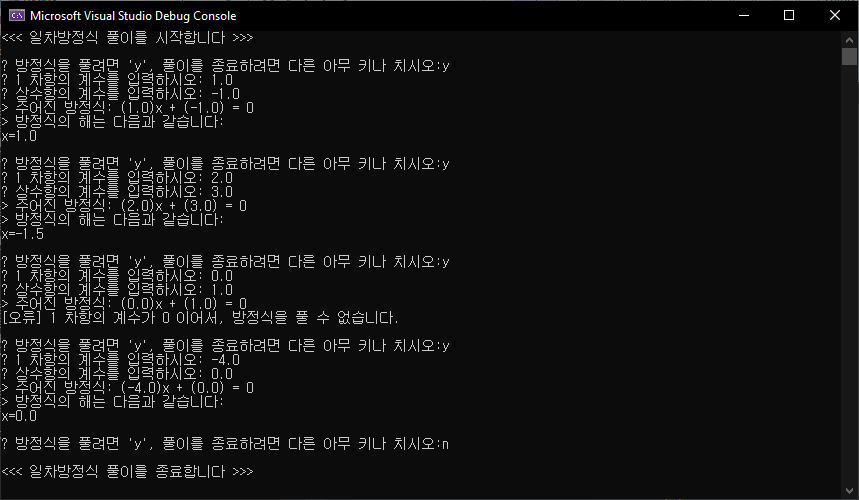
\includegraphics[width=\textwidth]{test_result.png}

    \subsection{입력과 출력}

    입력값은 실습 PPT에 제시된 예제를 따랐으며, 이에 따라 동일한 출력이 발생하였는 지를 확인하였음.

    \subsection{결과 분석}

    모든 테스트 입력과 출력에 대하여 정상임을 확인하였음. 
    
    \section{소스코드}
    전체 소스코드는 GitHub (0x00000FF/CNUCSE-Computer-Programming-III-2020-Spring) 에 업로드 되어 있으며, 제출시 본 보고서와 동봉되어 있다.
\end{document}

